\documentclass[10pt]{book}
\usepackage{url}
\usepackage{geometry}
\usepackage{multirow}
\usepackage{framed}
\usepackage{fancybox}
\usepackage[dvipdfmx]{graphicx}
\usepackage{color}
\usepackage{longtable}
\newenvironment{src}
{%begin
\VerbatimEnvironment
\begin{quote}
%\begin{screen}
\begin{Verbatim}
}
{%end
\end{Verbatim}
%\end{screen}
\end{quote}
}

\newcommand{\todo}[1]{\textcolor{red}{#1}}
\newcommand{\shtodo}[1]{\textcolor{blue}{#1}} % todos of sh

\begin{document}
\title{ {\bf {Xevolver XML Framework}}\\
A Framework for XML-Based AST Transformations \\
~\\
\bf{Introductory Tutorial (DRAFT)} \\
{(version @VERSION@)}}

\author{ {\bf Hiroyuki Takizawa} \\
Graduate School of Information Sciences\\
Tohoku University\\
Sendai 980-8579 Japan\\
+81-22-795-7010 (office)  +81-22-795-7011 (fax) \\
takizawa@cc.tohoku.ac.jp
       }
\date{\today}

\maketitle


\chapter*{Preface}

%  Purpose:
% \begin{itemize}
%    \item a. Welcome
%    \item b. Program features
%    \item c. Program benefits
% \end{itemize}
% \begin{center}
% *********************  \newline
% \end{center}
% \vspace{0.25in}


Welcome to the Xevolver XML introductory tutorial.  Xevolver
XML~(XevXML) is one of software products developed by the Xevolver
project.  The purpose of this project is to help migration of legacy HPC
applications to new systems by improving their performance portabilities
across system generations.  Since a high priority is given to
performance, an HPC application is often optimized and specialized for a
particular HPC system. As a result, the performance is not portable to
other systems.  To make matters worse, such system-specific code
optimizations are likely to be scattered over the application code. This
is one main reason why HPC application migration is so painful. It is
not affordable to reoptimize the whole code whenever a new system
becomes available.



XevXML is developed for XML-based AST transformations to provide an easy
way for user-defined code transformations.  The current implementation
of XevXML is built on top of the ROSE compiler framework. XevXML
converts ROSE's AST to an XML document, and exposes it to
programmers. So the programmers can use any XML-related technologies and
tools to transform the AST. Then, the transformed AST is given back to
the ROSE compiler framework so that the AST is unparsed to generate a
transformed application code.  Instead of directly modifying an
application code, programmers can define their own code transformations
to optimize the code for each system.  System-specific optimizations are
represented as XML translation rules, which can be defined separately
from an application code.  This leads to separation between application
requirements and system requirements, expecting a lower migration cost
of HPC applications to new systems.

\chapter*{Acknowledgments}

The Xevolver Project is supported by JST CREST Research Area
``Development of System Software Technologies for post-Peta Scale High
Performance Computing'' led by Dr.~Yonezawa at RIKEN AICS and later by
Dr.~Sato at RIKEN AICS.

XevXML is under active development yet, and many people are being
involved in the design and development.

Shoichi Hirasawa is a research associate employed by Tohoku University
for the Xevolver Project.  He has been actively working on writing
translation rules and testing XevXML tools. That is, he is always the
first user of the tools whenever new versions are committed to the code
repository.  His feedbacks are always helpful to improve the
tools. Moreover, he is the main author of most rules in the
transformation rule library. He designed the template of XSLT rules for
AST transformation.

There are many people I would like to thank for their contributions:
\begin{itemize}
 \item Contributing Collaborators: \\
       Reiji Suda~(The University of Tokyo),\\
       Yasuharu Hayashi~(NEC Corporation),\\
       Ryusuke Egawa~(Tohoku University),\\
       Daisuke Takahashi~(University of Tsukuba), and \\
       Kazuhiko Komatsu~(Tohoku University)

 \item Students: \\
       Chunyan Wang (Tohoku University),\\
       Xiong Xiao (Tohoku University), and \\
       Daichi Sato (Tohoku University)

 \item Advisory Boards:\\
       Hiroaki Kobayashi~(Tohoku University),\\
       Michael M. Resch~(HLRS),\\
       Wenmei W. Hwu~(UIUC), and\\
       Chisachi Kato~(The University of Tokyo)
\end{itemize}

%\noindent%


\tableofcontents
\chapter{Introduction}\label{cap:intro}

High-performance computing~(HPC) system architectures are getting more
complicated and diversified. Due to the system complexity, performance
optimizations specific to processor architectures, system
configurations, compilers, and/or libraries, called
\emph{system-specific optimizations}, are mandatory and becoming more
important to exploit the potential of a particular system; an
application code must be thoroughly optimized and specialized for one
platform to achieve high performance.  As a result, one HPC application
often needs to have multiple versions, each of which is optimized in a
different way for adapting to a particular platform.  The diversity of
system architectures increases the number of optimized versions required
for performance portability across major platforms.  To make matters
worse, popular platforms can change drastically, and thus an application
might need to be optimized not only for current major platforms but also
for future ones.  Accordingly, an increase in system complexity and
diversity would force a programmer to further invest enormous time and
effort for HPC application development and maintenance.

%The goal of the Xevolver project is to separate system-specific,
%system-aware performance optimizations from application codes.

%XevXML has been developed to express any code modifications separately
%from an application code. Practical HPC application development is a
%team work of multiple programmers.

XevXML~\cite{xevxml-hipc}~\cite{xevxml-sc13} is a code transformation
framework that allows users to define their own code transformations,
called \emph{user-defined code transformations}.  It exposes an
abstract syntax tree~(AST) to users so that they can apply any
transformations to the AST. Transformation rules written in external
files can be defined for individual systems, compilers, libraries, and
so on.  That is, code transformations representing system-aware
optimizations can be separated from an application code.  Hence, to
achieve high performance, the users no longer need to specialize an
application code for a particular platform.

XevXML assumes that an application code is annotated with a special
mark, using directives and/or comments, and transformations are applied
to the marked parts of the code.  Note that the mark indicates ``where
to transform,'' but does not indicate ``how to transform.''  The
transformation rules that indicate how to transform the code are defined
in external files. If system-aware code modifications are expressed as
code transformations, users can express system-awareness separately from
an application code.

As the name implies, XevXML employs eXtensible Markup
Language~(XML)~\cite{xml11} to represent an AST, i.e.,~an internal
representation of code structures used by compilers.  XML is a
widely-used data format, and various XML-related technologies and
tools have already been standardized and matured.  Therefore, the
users implement special code transformations by using only those
standard tools.  This chapter briefly describes an overview of code
transformation with XevXML.

\section{An overview of XevXML}
\begin{figure}[htb]
 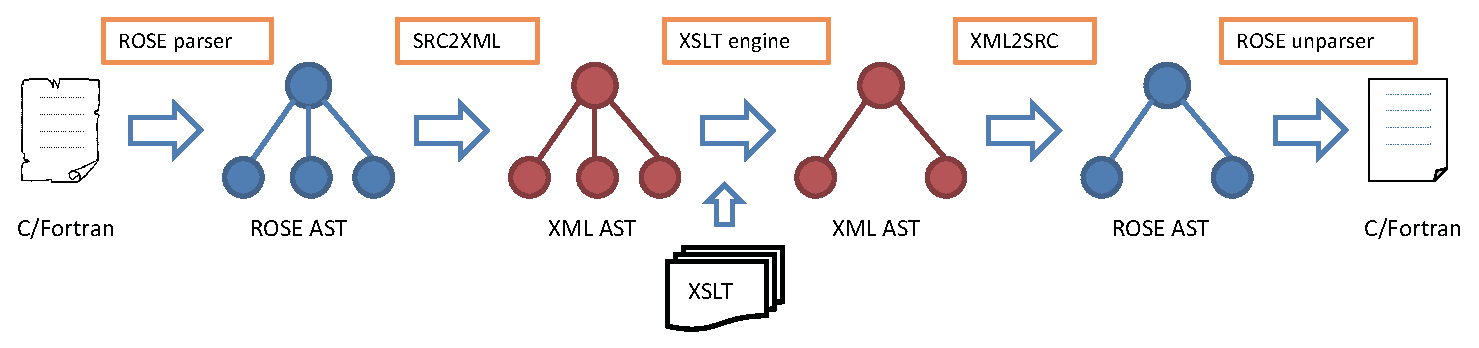
\includegraphics[width=\textwidth]{overview.eps}
 \caption{An overview of interconversion between ROSE ASTs and XML
 ASTs.}\label{fig:overview}
\end{figure}

XevXML has so far been developed on top of the ROSE compiler
infrastructure~\cite{rose}~\cite{quinlan2000rose}.  XevXML provides
the interconversion between an ROSE AST and its XML
representation. Figure~\ref{fig:overview} shows an overview of the
interconversion.  XevXML converts a ROSE AST to an XML representation
of the AST, called an \emph{XML AST}. In XevXML, an XML AST is exposed
to users.  After user-defined transformations, the transformed XML AST
is again converted back to a ROSE AST so that ROSE can unparse it to a
C or Fortran code.

The interconversion is achieved by combining the following two commands,
\texttt{src2xml} and \texttt{xml2src}.

\begin{framed}
\begin{description}
 \item[NAME]~\\
	    \texttt{src2xml} -- source-to-xml translator

 \item[SYNOPSIS]~\\
	    \texttt{src2xml [OPTIONS] INPUT-FILE}

 \item[DESCRIPTION]~\\ \texttt{src2xml} converts a C or Fortran code
	    into an XML document. \texttt{src2xml} reads a code from the
	    input file given by the command-line argument, and prints
	    an output XML document to the standard
	    output. 
	    \begin{description}
	    \item[\texttt{-F}, \texttt{--check\_fortran\_pragma}=$<$true/false$>$]
	    ~\newline enable the conversion of each Fortran pragma, e.g.~\texttt{!\$xev loog\_tag}, to an \texttt{$<$SgPragmaDeclaration$>$} element. This conversion is enabled by default, and needs to be disabled to make the behavior identical to that of ROSE. 
	    \item[\texttt{-h}, \texttt{--help}] ~\newline print the usage.
	    \end{description}
	    
	    \texttt{src2xml} also accepts some of ROSE command-line
	    options such as \texttt{-rose:verbose}. A ROSE
	    command-line option \texttt{-rose:skip\_syntax\_check} is
	    automatically appended to the command-line options because
	    it is required for some Fortran90 codes.

 \item[EXAMPLES]~\\ \texttt{src2xml hello.c $>$ hello.xml}\\ This command
	    will read \texttt{hello.c} and output its AST as an XML
	    document to \texttt{hello.xml}.
\end{description}
\end{framed}

\begin{framed}
\begin{description}
 \item[NAME]~\\
	    \texttt{xml2src} -- xml-to-source translator

 \item[SYNOPSIS]~\\
	    \texttt{xml2src [OPTIONS]}

 \item[DESCRIPTION]~\\ \texttt{xml2src} converts an XML AST to a C or
	    Fortran code. Since the original language, C or Fortran, is
	    recorded in an XML AST, \texttt{xml2src} generates a code
	    written in the original language. \texttt{xml2xml} reads an
	    XML AST from the standard input, and prints the generated
	    code to the standard output. At present, command-line
	    options for \texttt{xml2src} are simply ignored.

 \item[EXAMPLES]~\\ \texttt{xml2src $<$ hello.xml $>$ hello-again.c}\\
	    This command will read \texttt{hello.xml} and output its
	    code to \texttt{hello-again.c}.
\end{description}
\end{framed}

An XML AST is exposed to users. Thus, the users can apply any
transformation to the AST. As an AST is represented as an XML
document, any XML-related technologies and tools are available for the
transformations. XevXML employs XML Stylesheet Language
Transformation~(XSLT)~\cite{Kay08xslt}~\cite{Tidwell08xslt} as the
low-level interface to express the transformation rules of an XML AST.
AST transformation is what compilers do internally for code
transformation. Therefore, XevXML is capable of implementing various
code transformations.

XevXML can easily collaborate with ROSE.  ROSE already has various
features of code analyses and transformations to implement custom code
transformation programs in C++.  It must be painful if a user is
required to reimplement those features from scratch for XevXML. So
XevXML provides not only the above basic commands but also some C++
classes and functions, which are helpful to read and write XML ASTs, so
that code transformation programs developed with ROSE can handle XML
ASTs. Those classes and functions will be further described in
Chapter~\ref{chap:internal}.

If a code transformation is general enough and hence reusable in many
applications, it could be implemented using either ROSE or XevXML.
However, code transformations in practice could be application-specific,
system-specific, domain-specific, and even programmer-specific. If such
a code transformation program is implemented with ROSE, the user needs
to maintain the program in addition to his/her application code. In
XevXML, only transformation rules are defined declaratively, and code
transformations are performed using standard XML tools. So the user does
not need to develop his/her own program for applying the rules to
application codes.

%XevXML needs to be flexible enough to express various code
%transformations required in practical performance optimizations.

%If the user is familiar with ROSE, he/she can develop a code
%transformation by using ROSE.

%and write the result as an XML document.



\section{XML elements and attributes}\label{sec:xml}
Let's get started with a simple example, ``Hello, World!'' in C.
\begin{framed}
\begin{src}
#include <stdio.h>

int main()
{
  printf("Hello, World!\n");
  return 0;
}
\end{src}
\end{framed}


Using the \texttt{src2xml} command, the above code is converted to an
AST of the following XML document.

\begin{framed}
\begin{src}
<?xml version="1.0" encoding="UTF-8"?>
<SgSourceFile filename="hello.c" language="2" format="2">
  <SgGlobal>
    <SgFunctionDeclaration name="main"  end_name="0" >
        <SgTypeInt/>
      <SgFunctionParameterList/>
      <SgFunctionDefinition>
        <SgBasicBlock>
          <SgExprStatement>
            <SgFunctionCallExp>
              <SgFunctionRefExp symbol="printf" />
              <SgExprListExp>
                <SgCastExp mode="0" >
                    <SgPointerType base_type="SgModifierType" >
                      <SgModifierType modifier="const" >
                        <SgTypeChar/>
                      </SgModifierType>
                      <SgTypeChar/>
                    </SgPointerType>
                  <SgStringVal value="Hello, World!\n" paren="1"/>
                </SgCastExp>
              </SgExprListExp>
            </SgFunctionCallExp>
          </SgExprStatement>
          <SgReturnStmt>
            <SgIntVal value="0"  string="0" />
          </SgReturnStmt>
        </SgBasicBlock>
      </SgFunctionDefinition>
<PreprocessingInfo pos="2"  type="6" >
#include &lt;stdio.h&gt;

</PreprocessingInfo>
    </SgFunctionDeclaration>
  </SgGlobal>
</SgSourceFile>
\end{src}
\end{framed}

The data format of XML ASTs is designed so that the interconversion
between ROSE ASTs and XML ASTs becomes simple.  In general, an XML
document consists of XML elements and their attributes. In an XML AST,
each XML element corresponds to a ROSE AST node. XML attributes of an
XML element are used to keep the necessary information to restore the
ROSE AST node.  An XML AST looks like a text representation of a ROSE
AST.  In other words, XevXML provides another interface, XML, to handle
ROSE AST nodes.

In the above XML document, the first line just indicates that the file
is written in XML.  The root node of an AST is the \texttt{SgSourceFile}
element in the second line. The \texttt{SgSourceFile} element represents
the whole C code.  The \texttt{SgGlobal} element in the third line is a
child node of the root node, and indicates the global scope of the C
code. In the global scope, the \texttt{main} function is declared and
defined. In the function body, the first statement is an expression
statement, and the second statement is a \texttt{return}
statement. Comments and preprocessor information such as
\texttt{\#include $<$stdio.h$>$} are written as strings within the
\texttt{PreprocessingInfo} element.

XML attributes are used to restore ROSE AST nodes. For example, the
\texttt{SgStringVal} element corresponds to a ROSE AST node of a
\texttt{SgStringVal} class object representing a string.  Thus, a string
of \texttt{"Hello, World!$\backslash{}$n"} is written as its
\texttt{value} attribute. Similarly, the \texttt{SgFunctionRefExp}
element is a reference to the name of a function, and the function name
is given as the \texttt{name} attribute. Let's change ``printf'' is to
``puts'' by a text editor. Then, when the modified XML AST is converted
to a C code (by using the \texttt{xml2src} command), the function call
of \texttt{printf} will be changed to that of \texttt{puts}. This is a
simple example to show that, in XevXML, XML data transformation results
in AST transformation and thereby code transformation.

See the ROSE reference manual~\cite{rosemanual} to learn more about the
definition of each AST node.

\section{XML data transformation}\label{sec:xslt}

XML data are texts, and various tools are thus available to modify an
XML AST.  As shown in Section~\ref{sec:xml}, even a text editor can
modify an XML AST.  One may consider that, in the case of using a text
editor, modifying a C/Fortran code is much easier than modifying its XML
AST. So why don't we directly modify the code?  The answer is to avoid
specializing the code for a particular platform.

In many cases, system-aware code optimizations assuming a particular
target platform are necessary to exploit the system performance.  A
problem is that those optimizations are often harmful to the performance
of another platform.  A pragmatic approach is to maintain multiple
versions of a code, each of which is optimized for a different
platform. However, this results in degrading the maintainability and
making legacy application migration more painful.

%The modified AST can be converted back to a C or Fortran code.

XevXML has been developed to replace code modifications with
``mechanical transformations'' of an XML AST.  There are several
benefits of the replacement.  One important benefit is that the original
code is not necessarily specialized for a particular platform.  In other
words, system-awareness is separated from an application code.  This
will be helpful to avoid maintaining multiple versions of an application
code.

Another benefit is that expert knowledge about performance optimizations
can be expressed in a machine-usable way.  Basically, performance
optimizations are very intellectual tasks that are often done on a
case-by-case basis.  However, focusing on a particular case, there are
repetitive patterns in code modifications for performance
optimizations. Thus, the code modifications can be replaced with a
smaller number of mechanical code transformations.

The mechanical code transformations required instead of code
modifications could be application-specific, system-specific,
domain-specific, and even programmer-specific. Thus custom code
transformations are often needed for special demands of individual
cases.  Therefore, XevXML has been developed for users to define their
own code transformations in an easy way.

In XevXML, XSLT is currently employed to describe custom
transformation rules of XML ASTs at the lowest abstraction
level\footnote{Several high-level interfaces for definition of code
transformation rules are also under active development in the Xevolver
project.  One of such interfaces will be described in
Chapter~\ref{chap:json}.}  In XSLT, XML data transformations are
themselves written in XML.  XSLT uses XPath
expressions~\cite{xpath}~\cite{Kay08xslt}, to define a pattern within
a tree of XML elements and attributes.  During the transformation
process of XSLT, every XML element is visited in a depth-first manner.
When a pattern is found at an XML element, the XML element is altered
based on the rule associated with the pattern.

A simple XPath expression looks like a UNIX file path. In a UNIX file
system, files and directories organize a tree structure. A file path is
a text string to specify a location in the directory tree.  There are
two ways to point to the location of a file or a diretory.  One is an
absolute path, and the other is a relative path.  If the string of a
path starts with \texttt{/}, the path is an absolute path, otherwise it
is a relative path. An absolute path is the path to a file or a
directory from the root diretory. For example, the root directory is
expressed by \texttt{/}, its sub-directory named ``sub'' is expressed by
\texttt{/sub}, and a file named ``xfile'' that is located in the ``sub''
directory is expressed by \texttt{/sub/xfile}.  Note that \texttt{/}
represents the root directory and is also used as a delimiting
character.  On the other hand, a relative path indicates the path from
the working directory where a user or an application is located. When
the working diretory is \texttt{/sub}, a relative path to a
\texttt{xfile} can be represented as \texttt{xfile}, \texttt{./xfile},
\texttt{../sub/xfile}, etc.  Of course, those relative paths point to
the same location because \texttt{.} and \texttt{..} denote the working
diretory and its parent directory, respectively.

As well as a UNIX file path, an XPath expression also points to a
location in an XML document.  For example, the root of an XML document
is denoted by \texttt{/}.  A pattern in XML data is described by a
combination of XPath expressions.


An example of XSLT rules for AST transformation are as follows.
\begin{framed}
\begin{src}
<?xml version="1.0" encoding="UTF-8"?>
<xsl:stylesheet version="1.0"
   xmlns:xsl="http://www.w3.org/1999/XSL/Transform"
   xmlns:exslt="http://exslt.org/common">

  <xsl:template match="/">
    <xsl:apply-templates/>
  </xsl:template>

  <xsl:template match="*">
    <xsl:copy>
      <xsl:copy-of select="@*"/>
      <xsl:apply-templates/>
    </xsl:copy>
  </xsl:template>

  <xsl:template match="SgForStatement">
    <xsl:if test=".//*=SgForStatement">
    startLoopNest(); /* inserted */
    </xsl:if>
    <xsl:copy>
      <xsl:copy-of select="@*"/>
      <xsl:apply-templates/>
    </xsl:copy>
    <xsl:if test=".//*=SgForStatement">
    endLoopNest(); /* inserted */
    </xsl:if>
  </xsl:template>
</xsl:stylesheet>
\end{src}
\end{framed}
The above XML file defines three rules, each of which is described
within the \texttt{xsl:template} element. Based on these rules, an XML
document is transformed to another XML document, called an output XML
document.

The first rule matches the root of an XML document. The rule just
invokes \texttt{$<$xsl::apply-templates/$>$} that by default dictates to
visit all the sub-nodes and apply appropriate rules to them.

The second rule matches every XML element of an XML document, because
its XPath expression is given by a wild-card operator, \texttt{*}. The
rule is applied to an element unless a more specific rule matches the
element.  This rule simply copies the element and its attributes to the
output XML document.  The rule is recursively invoked because it invokes
\texttt{$<$xsl::apply-templates/$>$}.

The third rule matches only an \texttt{SgForStatement} element. It
checks if another \texttt{SgForStatement} element exists in the subtree
of the matched element.  Only if it exists, text data are inserted
before and after the matched element.

If the above XSLT rules are applied to an XML AST, two function calls,
\texttt{startLoopNest()} and \texttt{endLoopNest()}, are inserted before
and after each nested loop, and a single loop is unchanged as shown
below.
\begin{framed}
\begin{src}
beginLoopNest(); /* inserted */
for(i=0;i<N;i++){
  for(j=0;j<M;j++){
    /* loop body 1 */
  }
}
endLoopNest();  /* inserted */

for(j=0;j<M;j++){
 /* loop body 2 */
}
\end{src}
\end{framed}
This is an example of text insertion based on code pattern matching.
Although this kind of rule is useful in practice, more advanced code
transformations can be achieved by writing XSLT rules because XSLT can
change the structure of an XML AST.  Chapter~\ref{chap:xslt} will
describe how to write XSLT rules for AST transformation.

Although users can use any XSLT processor for code transformation,
XevXML provides the \texttt{xsltexec} command for XSLT-based code
transformation. In general, an XSLT file can import XSLT rules defined
in other XSLT files. If a specified file written in an XSLT file for
importing rules does not exist in the working directory, the
\texttt{xsltexec} command looks for the file in the XevXML
transformation library path specified by an environment variable,
\texttt{XEVOLVER\_LIBRARY\_PATH}. The library path would usually be
specified so that the command uses predefined XSLT rules offered by
XevXML.  The command also has a command line option to specify the
library path.

\begin{framed}
\begin{description}
 \item[NAME]~\\
	    \texttt{xsltexec} -- a simple XSLT processor for XevXML

 \item[SYNOPSIS]~\\
	    \texttt{xsltexec [OPTIONS] XSLT-FILE}

 \item[DESCRIPTION]~\\ \texttt{xsltexec} applies XSLT rules to an XML
	    representation of an AST, called an XML AST. XSLT rules are
	    defined in a file given by the command-line argument. In the
	    XSLT file, predefined XSLT rules offered by XevXML are also
	    available without specifying the absolute paths of the XSLT
	    files installed to the system.

	    The command reads an input XML AST from the standard input,
	    and prints an output XML AST to the standard output. The
	    command-line options are as follows.

	    \begin{description}
	    \item[\texttt{-L}, \texttt{--libdir}=$<$path$>$]~\newline
	    specify the library path.      
    	    \item[\texttt{-h}, \texttt{--help}]~\newline
	    print the usage.
	    \end{description}

	    An environment variable, \texttt{XEVOLVER\_LIBRARY\_PATH},
	    is used to configure the default path of the transformation
	    library.
 \item[EXAMPLES]~\\ \texttt{xsltexec sample.xsl $<$ hello.xml}\\ This
	    command will read an XML AST in \texttt{hello.xml} and
	    transform the AST based on the XSLT rules defined in
	    \texttt{sample.xsl}. The transformed AST is printed out to
	    the standard output.
\end{description}
\end{framed}

%It is hence necessary to easily define such specific code
%transformations.

%it is not easy for standard programmers to develop special code
%translators using compiler tools such as ROSE.

\section{Summary}
This chapter describes an overview of the XevXML framework. Then, three
basic commands, \texttt{src2xml}, \texttt{xml2src}, and
\texttt{xsltexec}, are introduced for user-defined code transformations
with XML specifications and tools. Using some simple examples,
interconversion between ROSE ASTs and XML ASTs is explained, and also
simple transformations are shown in this chapter.

%To be described.
\chapter{User-Defined Directives}\label{chap:json}

%XevXML is a framework for user-defined code transformations.

In XevXML, transformation rules are defined by XSLT rules, and applied
to an XML AST. By writing appropriate XSLT rules, XevXML as well as
compilers can transform an AST in various ways.  However, directly
transforming an AST might be a too low-level approach for performance
optimizations on a case-by-case basis.  Therefore, several high-level
interfaces for XevXML are under development.

In practice, code modifications for performance optimizations are often
expressed by combinations of well-known loop transformations.  Moreover,
text insertion and deletion based on code pattern matching are also
frequently required for practical performance optimizations.
Nonetheless, it is not very easy to correctly define their XSLT rules
manually.

In this chapter, a high-level interface for user-defined code
transformations is described. The interface is designed only for some
specific purposes.  Although the interface is less flexible than the
XSLT approach of straightforwardly dictating AST transformations, it
offers an easy way to quickly define a custom compiler directive that is
associated with a composite of predefined rules. Such a directive can
also be associated with text insertion and deletion. Therefore, the
high-level interface is useful for generating a lot of transformation
rules and also for mechanically inserting some texts into a code, which
are frequently required in practical performance optimizations.

\section{XSLT rule generation}
XevXML provides the \texttt{xsltgen} command that reads a simple
JSON\cite{json} file to generate XSLT rules, each of which is associated
with one user-defined compiler directive.  An XSLT rule generated by
\texttt{xsltgen} is either a composite of predefined XSLT rules or text
insertion/deletion.  Although \texttt{xsltgen} is available only for
these purposes, it provides a much easier way to define a custom
compiler directive associated with such a rule.

\begin{framed}
\begin{description}
 \item[NAME]~\\
	    \texttt{xsltgen} -- XSLT rule generator

 \item[SYNOPSIS]~\\
	    \texttt{xsltgen [OPTIONS] }

 \item[DESCRIPTION]~\\ \texttt{xsltgen} converts a configuration file in
	    JSON to an XSLT file of code transformation rules.
	    \texttt{xsltgen} reads a JSON file from the standard input,
	    and prints a XSLT file to the standard
	    output.

 \item[EXAMPLES]~\\ \texttt{xsltgen $<$ config.json $>$ rules.xsl}\\ This command
	    will read \texttt{test.json} and write XSLT rules to \texttt{rules.xsl}.
\end{description}
\end{framed}

An example of a JSON file is as follows.
\begin{framed}
\begin{src}
{
  "xev loop_tag1":{
    "target":"SgIfStmt",
    "insert-before":"!$test"
  }
  "xev loop_tag2":{
    "target":"SgFortranDo",
    "rules":[
      {"chillUnrollJam":{"loopName":"k","factor":4}},
      {"chillUnroll":{"loopName":"i","factor":2}}
    ]
  }
}
\end{src}
\end{framed}

A JSON object enclosed in \texttt{\{} and \texttt{\}} is an unordered
collection of any values. The root object whose \texttt{\{} is in the
first line contains two pairs of keys and values that are directive
definitions.  Notice that the colon character, \texttt{:}, is used to
separate a key and its value. In a directive definition, the key
indicates the directive name, and its value is a JSON object, called a
rule definition, that defines the rule associated with the directive.
In the above file, two compiler directives, \texttt{xev loop\_tag1} and
\texttt{xev loop\_tag2}, are defined for Fortran. If the key is
\texttt{"*"}, the rule defined by its value is applied without any
directive. The pair whose key is \texttt{"target"} specifies what kind
of statements the rule is applied. That is, the value is expected to be
the AST node name of the statement that appears after the directive.

The first directive, \texttt{xev loop\_tag1}, assumes that it is
followed by an \texttt{IF} statement. Then, it simply inserts a comment
before the IF statement.

The second directive, \texttt{xev loop\_tag2}, is associated with a
composite of two predefined rules, \texttt{chillUnrollJam} and
\texttt{chillUnroll}.  This directive applies those loop optimization
rules with the given parameters to the \texttt{DO} statement following
the directive, which is an XML element of \texttt{SgFortranDo}.  The
predefined rules with their parameters are listed in an array of JSON,
which is enclosed in \texttt{[} and \texttt{]}. Unlike an object of
JSON, an array is an ordered list. The rules are applied in the same
order as they appear in the array.

\section{Loop optimization}
The most time-consuming part of a scientific application is usually
written as a loop, a so-called kernel loop.  Thus, loop optimization is
a key to improve the performance of such an application.  There are a
lot of loop optimization techniques, and most of them are supposed to be
done by compilers. Typical loop optimization techniques are as follows.
\begin{itemize}
 \item Loop unrolling
 \item Loop tiling
 \item Loop interchange
 \item Loop permutation
 \item Loop collapse
 \item Loop fusion
 \item Loop fission~(aka. loop distribution)
 \item Unroll and jam~(aka. outer loop unrolling)
\end{itemize}

In some cases, compilers are unable to perfectly apply those techniques
to a kernel loop for various reasons.  In such a case, manual
optimizations of the kernel loop might be required to achieve high
performance. However, even if the optimization is a certain combination
of the techniques listed above, manual optimization of a kernel loop is
not an easy task. This is because an appropriate combination of loop
optimization techniques is unknown. In addition, most of loop
optimization techniques have some parameters that need to be determined
appropriately for high performance.

To make matters worse, different platforms require different loop
optimizations.  Appropriate loop optimization, i.e.,~the combination and
parameters, could change drastically depending on the target platform.
Thus, manual code modification for loop optimization generally results
in specializing the code only for a particular platform. Accordingly,
the necessary information for loop optimizations should be separated
from an application code.

Because of the importance, XevXML provides the \texttt{xsltgen} command
as an easy way to compose loop optimization techniques and to associate
the composite with a user-defined compiler directive.  Code
transformation rules for basic loop optimization techniques are
predefined. The predefined rules in the XevXML transformation rule
library are listed in Section~\ref{sec:predef}.

%\textbf{*** List of predefined rules and their parameters***}

Those predefined rules are themselves written in XSLT, and hence
customizable for special demands of individual cases. A customized rule
can also be used together with other predefined rules using the
\texttt{xsltgen} command. Chapter~\ref{chap:xslt} describes how to
customize predefined rules and also how to define new rules.


\section{Text insertion/deletion}
The \texttt{xsltgen} command can also be used to define a custom
compiler directive for inserting or deleting a text into a code. Such a
directive is useful to literally change some statements depending on the
target platform.  Although the C preprocessor can also achieve it using
\texttt{\#ifdef}, such an approach often makes an application code
unmaintainable, so-called \texttt{\#ifdef} hell. In the case of using
\texttt{xsltgen}, the text to be inserted is written in an external
file, which is an XSLT file generated by \texttt{xsltgen}.  Therefore,
the original code is not messed up with platform-dependent code
fragments.

To define a directive for text insertion, a JSON object of the directive
definition has one or more pairs whose keys are
\texttt{"insert-before"}, \texttt{"insert-after"}, or \texttt{"replace"}
and whose values are strings. As the names imply,
\texttt{"insert-before"}, \texttt{"insert-after"}, and
\texttt{"replace"} inserts a text before the target statement, inserts a
text after the target statement, and replace the target statement with a
text, respectively.

For example, the following JSON file will produce an XML rule that
inserts the function calls before and after a \texttt{for} loop.
\begin{framed}
\begin{src}
{
  "*":{
    "target":"SgForStatement",
    "insert-before":"startLoop();",
    "insert-after":"endLoop();"
  }
}
\end{src}
\end{framed}
In the above directive definition, the directive name is \texttt{*}. The
rule does not need any directive in the code, and is applied to every
\texttt{for} statement. More specifically, the rule is applied to the
AST subtree whose root is \texttt{SgForStatement}. Therefore, the
function call of \texttt{endLoop();} is inserted right after the loop
body of every \texttt{for} loop.

If a pair of \texttt{"replace"} and an empty string is given in the
directive definition, the directive will simply remove the target
statement. Namely, such a directive can be used to remove the statement
for a particular platform.


\section{Summary}
The \texttt{xsltgen} command is now under active development to provide
a high-level interface for users to compose predefined loop
optimizations.  Although it is currently used only for some specific
purposes, it offers a very easy way to define a user-defined code
transformation associated with a custom directive. Therefore, it will be
further extended to allow users to quickly define various kinds of code
transformations.

\chapter{AST Transformation Rules}

XevXML represents an AST in an XML format, and various XML tools are
hence available for AST transformation. In XevXML, the transformation
rules are (internally) represented as XSLT rules. In a special code
transformation is needed, the most flexible and expressive way is to
write an XSL rule for the transformation.

XevXML provides a lot of predefined rules that are also written in XSLT.
Users can customize those predefined rules for their own
purposes. XevXML also provides an XSLT rule template as a sample for
users to newly define their special transformation rules.

This chapter describes how to define and customize an XSLT rule for AST
transformation in XevXML.


\chapter{Internal Structures and Behaviors}\label{chap:internal}

Since ROSE already has various features of code analyses and
transformations useful to implement custom code transformation programs,
XevXML provides some C++ classes and functions, which are helpful for
such programs to read and write XML ASTs.  As a result, code
transformation programs developed with ROSE can handle XML ASTs.

This chapter describes XevXML classes and functions that allows ROSE to
handle XML ASTs. By inheriting the classes, users can develop customized
versions of \texttt{src2xml} and \texttt{xml2src} commands. For example,
\texttt{src2xml} would be customized so that some additional XML
attributes are written in an XML AST.


\section{Utility functions}
%A simplified version of the code is as follows.

%A minimum code of a ROSE-based translator is as follows.
By using ROSE, it is easy to write an identity translator, i.e.,~the
simplest translator.
\begin{framed}
\begin{src}
/* identity.cpp */
#include <rose.h>

int main(int argc,char** argv){
  SgProject* sageProject=frontend(argc,argv);

  /* do something here for code transformation */

  return backend(sageProject);
}
\end{src}
\end{framed}

The \texttt{frondend()} function reads a code and builds its AST. The
\texttt{backend()} function passes the AST to the backend for unparsing
and compilation.

XevXML offers a utility function, \texttt{XevConvertRoseToXml()}, for
such a ROSE-based translator to print out a ROSE AST as an XML AST. All
of the functions and classes provided XevXML are defined within a name
space, \texttt{XevXml}.


For example, a simplified version of the \texttt{src2xml} command is as
follows. It just prints out an XML AST, and then immediately ends.

\begin{framed}
\begin{src}
/* simple.cpp */
#include <iostream>
#include <rose.h>
#include <xevxml.hpp>

int main(int argc,char** argv){
  SgProject* sageProject=frontend(argc,argv);

  /* print out an XML AST to the standard output */
  XevXml::XevInitialize();
  XevXml::XevConvertRoseToXml(std::cout,&sageProject);
  XevXml::XevFinalize();

  /* return backend(sageProject); */
  return 0; /* backend is not called in this example */
}
\end{src}
\end{framed}

Run your compiler with appropriate options to specify the paths to
necessary header files and libraries.

\vspace{5mm}
\texttt{\% g++ -I... simple.cpp -o simple -L... -lxevxml -lrose -lxalan-c -lxerces-c }
\vspace{5mm}

\noindent The generated executable, \texttt{simple}, will print out an
XML AST of a C or Fortran code to the standard output.

\vspace{5mm}
\texttt{\% ./simple input.c}
\begin{verbatim}
<?xml version="1.0" encoding="UTF-8"?>
<SgSourceFile file="input.c" lang="2" fmt="2">
 <SgGlobal>
 ...omitted...
 </SgGlobal>
</SgSourceFile>
\end{verbatim}
\vspace{5mm}

A simplified version of the \texttt{xml2src} command is as follows.

\begin{framed}
\begin{src}
/* simple2.cpp */
#include <iostream>
#include <rose.h>
#include <xevxml.hpp>

int main(int argc,char** argv){
  SgProject* sageProject=0;

  /* read an XML AST from the standard input */
  XevXml::XevInitialize();
  if( XevXml::XevConvertXmlToRose(std::cin,&sageProject) == false ){
    std::cerr << " failed" << std::endl;
    abort();
  }
  else {
    /* check the AST (optional) */
    AstTests::runAllTests(sageProject);
    /* unparse the AST and print it out */
    XevXml::XevUnparseToStream(std::cout,&sageProject);
  }
  XevXml::XevFinalize();

  return 0;
}
\end{src}
\end{framed}

The \texttt{XevConvertXmlToRose()} function reads an XML AST and
converts it to a ROSE AST. If the conversion does not fail, the
\texttt{XevUnparseToStream()} function is called to print the ROSE AST
to a C++ stream.  Accordingly, the above code, \texttt{simple2}, reads
an XML AST from the standard input, and then unparses it. The unparsed
code is printed out to the standard output.

The following combination of the above two commands works as an identity
translator.

\vspace{5mm}
\texttt{\% ./simple input.c | ./simple2 }
\begin{verbatim}
#include <stdio.h>

int main()
{
  ...omitted...
  return 0;
}
\end{verbatim}


The behaviors of the \texttt{XevConvertRoseToXml()} function can be
changed using a \texttt{XevXmlOption} class object. For example, a
slightly-modified vetsion of \texttt{simple.cpp} that uses the
\texttt{XevXmlOption} is as follows.
\begin{framed}
\begin{src}
/* simple-mod.cpp */
#include <iostream>
#include <rose.h>
#include <xevxml.hpp>

int main(int argc,char** argv){
  SgProject* sageProject=frontend(argc,argv);

  /* print out an XML AST to the standard output */
  XevXml::XevInitialize();
  XevXml::XevXmlOption opt;
  /* the following options are disabled by default */
  opt.getFortranPragmaFlag() = true; // parse Fortran pragmas
  opt.getPrintAddressFlag() = true; // print the address of every AST node

  /* execute the conversion with the above options */
  XevXml::XevConvertRoseToXml(std::cout,&sageProject,&opt);
  XevXml::XevFinalize();

  return 0;
}
\end{src}
\end{framed}

In the above code, all the options disabled by default are enabled.  By
default, every ``xev pragma'' in a Fortran code, which starts with
\texttt{!\$xev}, is handled as a comment.  By enabling the flag accessed
by the \texttt{getFortranPragmaFlag()} method, such a pragma will be
converted to an XML element. The other options are basically used for
debugging.

\section{Visitor classes}

As described in the previous section, a C code whose file name is
\texttt{input.c} will be converted to the following XML AST.
\vspace{5mm}
\begin{verbatim}
<?xml version="1.0" encoding="UTF-8"?>
<SgSourceFile file="input.c" lang="2" fmt="2">
 <SgGlobal>
 ...omitted...
 </SgGlobal>
</SgSourceFile>
\end{verbatim}
\vspace{5mm}
ROSE uses C++ class objects, called \emph{Sage III class objects}, to
represent nodes of an AST.  That is, every node of a ROSE AST is an
object of a Sage III class. Each Sage III class is a subclass of the
\texttt{SgNode} class.  For example, the \texttt{SgGlobal} class is one
Sage III class, and its object represents the global scope of a code.
On the other hand, every node of an XML AST is an XML element whose name
is the same as the Sage III class name of its corresponding ROSE AST
node.  Hence, an \texttt{$<$SgGlobal$>$} element appears right after an
\texttt{$<$SgSourceFile$>$} element, which corresponds to an
\texttt{SgSourceFile} class object representing the source code.  See
the ROSE reference manual\cite{rosemanual} for more details of Sage III
classes. Chapter~\ref{sec:attrib} also describes XML elements of Sage
III classes currently supported by XevXML.

XML attributes are used to keep the necessary information to rebuild
each ROSE AST. For example, \texttt{$<$SgSourceFile$>$} has a
\texttt{lang} attribute so that an XML AST can record the language of
the original source code.  The attributes of XML AST nodes are described
in Chapter~\ref{sec:attrib}.

To customize the format of an XML AST, XevXML offers two internal C++
classes, \texttt{XevSageVisitor} and \texttt{XevXmlVisitor}.  The former
class traverses an AST of Sage III classes used in ROSE, and translates
it to an XML AST.  The latter traverses an XML AST to rebuild ROSE's
AST.

The \texttt{XevConvertRoseToXml()} function internally uses the
\texttt{XevSageVisitor} class for converting a ROSE AST to an XML AST.
The \texttt{XevSageVisitor} class is a Vistor pattern class that visits
every node of a ROSE AST in a depth-first fashion. Whenever
\texttt{XevSageVisitor} visits an AST node, it writes an XML element
whose name is the same as the Sage III class name of an AST node, e.g.,
\texttt{SgGlobal}.  When writing XML attributes of each XML element,
\texttt{attribSg*()} method is invoked (\texttt{Sg*} is the name of a
Sage III class). Similarly, when writing the sub-nodes of each XML
element, \texttt{inodeSg*()} method is invoked.  Therefore, by
overloading those methods, a user can customize XML documents generated
by the \texttt{XevSageVisitor} class.

In the following code, a new attribute \texttt{"foo"} whose value is
\texttt{"bar"} is added to an \texttt{$<$SgGlobal$>$} element.
\begin{framed}
\begin{src}
/* custom.cpp */
#include <xevxml.hpp>

class MyVisitor: public XevXml::XevSageVisitor
{
public:
  MyVisitor():XevXml::XevSageVisitor() {}

  void attribSgGlobal(SgNode* node)
  {
    // print the default attributes
    XevXml::XevSageVisitor::attribSgGlobal(node);
    std::ostream& os = getOutputStream();

    os << " foo=\"str\"";
    os << " bar=\"1\"";
  }
};

int main(int argc,char** argv)
{
  SgProject* sageProject=frontend(argc,argv);
  MyVisitor visitor;
  XevXml::XevXmlOption opt;

  XevXml::XevInitialize();
  visitor.setXmlOption(&opt);
  visitor.write(std::cout,&sageProject);
  XevXml::XevFinalize();
  return 0;
}
\end{src}
\end{framed}

The \texttt{MyVisitor} class is a subclass of \texttt{XevSageVisitor}.
The \texttt{XevSageVisitor::setXmlOption()} method is used to pass an
\texttt{XevXmlOption} object to the \texttt{MyVisitor} class
object. After that, the \texttt{XevSageVisitor::write()} method is
invoked to write an XML AST to a given \texttt{std::ostream} object.

The \texttt{XevSageVisitor::attribSgGlobal()} method is overloaded by
\texttt{MyVisitor::attribSgGlobal()}.  In the new method, the reference
to an \texttt{std::ostream} object, which is given by the first argument
of the \texttt{XevSageVisitor::write()} method,
i.e.,~\texttt{std::cout}, is obtained by calling
\texttt{getOutputStream()}.  Then, two strings are passed to the object.
As a result, the strings appear as XML attributes of an
\texttt{$<$SgGlobal$>$} element.

\vspace{5mm}
\texttt{\% ./custom input.c}
\begin{verbatim}
<?xml version="1.0" encoding="UTF-8"?>
<SgSourceFile file="input.c" lang="2" fmt="2">
 <SgGlobal foo="str" bar="1">
 ...omitted...
 </SgGlobal>
</SgSourceFile>
\end{verbatim}
\vspace{5mm}

The \texttt{XevConvertXmlToRose()} function internally uses the
\texttt{XevXmlVisitor} class for converting an XML AST to a ROSE AST.
The \texttt{XevXmlVisitor} class is a Vistor pattern class that visits
every node of an XML AST in a depth-first fashion.  Whenever
\texttt{XevXmlVisitor} visits an XML element, \texttt{visigSg*()} method
is invoked. Therefore, by overloading such a method, a user can
customize the rebuilding process of an AST.

\begin{framed}
\begin{src}
/* custom2.cpp */
#include <xevxml.hpp>
#include <xmlutils.hpp>

class MyXmlVisitor: public XevXml::XevXmlVisitor
{
public:
  SgNode* visitSgGlobal(xercesc::DOMNode* node, SgNode* parent)
  {
    SgNode* n =
      XevXml::XevXmlVisitor::visitSgGlobal(node,parent);

    std::string sval;
    if(XevXml::XmlGetAttributeValue(node,"foo",&sval)==true){
      std::cerr << " attribute \"foo\" is found" << std::endl;
      std::cerr << " the value is " << sval << std::endl;
    }
    else {
      std::cerr << " attribute \"foo\" is not found" << std::endl;
    }

    int ival;
    if(XevXml::XmlGetAttributeValue(node,"bar",&ival)==true){
      std::cerr << " attribute \"bar\" is found" << std::endl;
      std::cerr << " the value is " << ival << std::endl;
    }
    else {
      std::cerr << " attribute \"bar\" is not found" << std::endl;
    }

    float fval;
    if(XevXml::XmlGetAttributeValue(node,"baz",&fval)==true){
      std::cerr << " attribute \"baz\" is found" << std::endl;
      std::cerr << " the value is " << fval << std::endl;
    }
    else {
      std::cerr << " attribute \"baz\" is not found" << std::endl;
    }

    return n;
  }
};

int main(int argc,char** argv)
{
  SgProject* sageProject=0;
  MyXmlVisitor visitor;
  XevXml::XmlInitialize();
  visitor.read(std::cin,&sageProject);
  XevXml::XmlFinalize();
  return 0;
}
\end{src}
\end{framed}

When an XML AST is traversed, every XML element is represented as an
\texttt{xercesc::DOMNode} class object. Because of the depth-first AST
traversal, its parent node is already converted to an \texttt{SgNode}
object in many cases.  The pointers to those two objects are given to
\texttt{XevXmlVisitor::visitSg*()} as function arguments.  If the
\texttt{SgNode} object of the parent node is not available yet, the
second argument is \texttt{NULL}.

\texttt{XevXmlVisitor::visitSg*()} has to return a pointer to an
\texttt{SgNode} object, which is actually an \texttt{Sg*} object.  For
example, the \texttt{XevXmlVisitor::visitSgGlobal()} method is called
when a \texttt{$<$SgGlobal$>$} element is visited.  This method and its
overloaded versions are expected to return a pointer to an
\texttt{SgGlobal} object.

In the above code, \texttt{XevXmlVisitor::visitSgGlobal()} is overloaded
by the \texttt{MyXmlVisitor} class so that a utility function,
\texttt{XevXml::XmlGetAttributeValue()}, is called for checking if each
attribute is given or not.  Here,
\texttt{XevXml::XmlGetAttributeValue()} is a C++ template function
defined in \texttt{xmlutils.hpp}.

\begin{verbatim}
% ./custom input.c |./custom2
 attribute "foo" is found
 the value is str
 attribute "bar" is found
 the value is 1
 attribute "baz" is not found
\end{verbatim}

\section{Summary}
XmlXML is an extensible code transformation framework. Its internal
structures and behaviors can be customized if necessary. The utility
functions and classes will be useful to develop tools for
transformation, visualization, and analysis of an XML AST. Use of XML
for representing an AST will by design be helpful to make those tools
interoperable.

%The interoperability is one important benefit of using XevXML.


\chapter{Installation}\label{chap:app}


\section{Requirements}

\begin{itemize}
 \item ROSE compiler infrastructure -- \url{http://rosecompiler.org/}
 \item Apache Xerces C++ 3.1.1 -- \url{http://xerces.apache.org/}
 \item Apache Xalan C++ 1.0 -- \url{http://xml.apache.org/xalan-c/}
 \item PicoJSON -- \url{https://github.com/kazuho/picojson/}
\end{itemize}




\section{Installation guide}
\begin{enumerate}
 \item First of all, some environment variables such as
       \texttt{LD\_LIBRARY\_PATH}, \texttt{JAVA\_HOME}, and \texttt{CXX}
       must be correctly set so as to use ROSE, Xerces, and Xalan.


 \item Create a new directory at the top diretocry for building the package.

       \vspace{5mm}
       \texttt{\% mkdir mybuild}

       \texttt{\% cd mybuild}
       \vspace{5mm}

 \item Run the \texttt{cmake} command at the created directory to
       generate Makefile and copy necessary files.

       \vspace{5mm}
       \texttt{\% cmake ../}
       \vspace{5mm}

       The \texttt{cmake} command accepts various options. For example,
       the install diretory is changed by using the
       \texttt{-DCMAKE\_INSTALL\_PREFIX} option.

       \vspace{5mm}
       \texttt{\% cmake -DCMAKE\_INSTALL\_PREFIX=/usr/local/xevxml ../}
       \vspace{5mm}

       If you need to use a specific version of a library or a header
       file, you can also use environment variables
       \texttt{CMAKE\_LIBRARY\_PATH} and \texttt{CMAKE\_INCLUDE\_PATH}.
       For example, if you need to use a library or a header file in
       \texttt{/home/user/local}, define those enviromnent variables as
       follows.

       \vspace{5mm}
       \texttt{\% export CMAKE\_LIBRARY\_PATH=/home/user/local/lib:\$CMAKE\_LIBRARY\_PATH}

       \texttt{\% export CMAKE\_INCLUDE\_PATH=/home/user/local/include:\$CMAKE\_INCLUDE\_PATH}
       \vspace{5mm}

      Those environment variables must be correctly set so that all of
      the necessary header files and libraries such as
      \texttt{picojson.h} and \texttt{rose.h} are found by the
       \texttt{cmake} command.

       See the \texttt{cmake} manual for more details~\cite{cmake}.

 \item Run the GNU make command.

   To compile the package,

       \vspace{5mm}
       \texttt{\% make}
       \vspace{5mm}

   To install the package,

       \vspace{5mm}
       \texttt{\% make install}
       \vspace{5mm}

   To test the package,

       \vspace{5mm}
       \texttt{\% make test}
       \vspace{5mm}

       Some of tests will be failed. But it does not necessarily mean
       that something is wrong with the built binaries. Even if
       everything goes well, XevXML fails in some tests. This is mainly
       because XevXML is built on top of ROSE and unable to pass the
       tests if ROSE cannot properly parse/unparse the test codes.

\end{enumerate}


\appendix
\chapter{XML elements and their attributes}\label{sec:attrib}

\section{Class hierarchy}
\begin{verbatim}
SgNode -+- SgStatement   -+- SgDeclarationStatement
        |
        +- SgExpression  -+- SgBinaryOp
        |                 |
        |                 +- SgUnaryOp
        +- SgType         |
        |                 +- SgValueExp
        +- SgSupport 
\end{verbatim}
\section{Statements}
This section describes XML elements of \texttt{SgStatement} subclasses
currently supported by XevXML.  

\subsection{XML elements}
All XML elements of \texttt{SgStatement} subclasses are described below.
If an XML element of a \texttt{SgStatement} subclass has its own XML
attributes, the attributes are also listed in the description.
\begin{longtable}[l]{l|p{10cm}}
 \hline
 XML element name & Description \\
 \hline\hline
 \endfirsthead
 \multicolumn{2}{l} {(continued)}\\
 \hline
 XML element name & Description \\
 \hline\hline
 \endhead
 \hline
 \multicolumn{2}{r} {(continue to next page)}\\
 \endfoot
 \hline
 \endlastfoot
 \multicolumn{2}{l}{Declarations}\\
 \hline
 \texttt{SgAsmStmt}& asm statement (not tested)\\
 & ~\texttt{code} (string): assembly code \\
 & ~\texttt{volatile} (int): 0 (not volatile) or 1 (volatile)\\
\texttt{SgAttributeSpecificationStatement}& attribute specification (Fortran only)\\
 & ~\texttt{kind} (int): See Section~\ref{sec:stmtatt}.\\
 %& ~~~\texttt{SgAttributeSpecificationStatement::attribute\_spec\_enum}\\
 \texttt{SgClassDeclaration}& declaration of a class or a structure\\
 & ~\texttt{name} (string): class name\\
 & ~\texttt{type} (int): 0 (class), 1 (struct), or 2 (union)\\
 \texttt{SgCommonBlock}& COMMON block (Fortran only)\\
 \texttt{SgContainsStatement}& CONTAINS statement (Fortran only)\\
 \texttt{SgDerivedTypeStatement}& derived type declaration (Fortran only)\\
 & ~\texttt{name} (string): derived type name\\
 & ~\texttt{type} (int): 0 (class), 1 (struct), or 2 (union)\\
 \texttt{SgEntryStatement}& ENTRY statement (Fortran only)\\
 & ~\texttt{name} (string): entry name\\
 & ~\texttt{result} (string): result variable name\\
 \texttt{SgEnumDeclaration}& enum declaration\\
 & ~\texttt{name} (string): enum name\\
 \texttt{SgEquivalenceStatement}& EQUIVALENCE statement (Fortran only)\\
 \texttt{SgFormatStatement}& FORMAT statement (Fortran only)\\
 \texttt{SgFortranIncludeLine}& INCLUDE (Fortran only)\\
 & ~\texttt{filename} (string): filename name\\
 \texttt{SgFunctionDeclaration}& function declaration \\
 & ~\texttt{name} (string): function name\\
 & ~\texttt{end\_name} (int): \texttt{set\_named\_in\_end\_statement()}\\
 \texttt{SgFunctionParameterList}& function parameter list\\
 \texttt{SgImplicitStatement}& IMPLICIT statement (Fortran only)\\
 \texttt{SgInterfaceStatement}& INTERFACE statement (Fortran only)\\
 & ~\texttt{name} (string): interface name\\
 & ~\texttt{type} (int): \texttt{SgInterfaceStatement::generic\_spec\_enum}\\
 \texttt{SgModuleStatement}& MODULE statement (Fortran only)\\
 & ~\texttt{name} (string): module name\\
 & ~\texttt{type} (int): 0 (class), 1 (struct), or 2 (union)\\
 \texttt{SgNamelistStatement}& NAMELIST statement (Fortran only)\\
 & ~\texttt{group} (string): group name\\
 \texttt{SgPragmaDeclaration}& pragma declaration\\
 \texttt{SgProcedureHeaderStatement}& procedure declaration (Fortran only)\\
 & ~\texttt{name} (string): procedure name\\
 & ~\texttt{kind} (int): subprogram kind\\
 & ~\texttt{result} (string): result variable name\\
 & ~\texttt{pure} (int): 0 (not pure) or 1 (pure)\\
 & ~\texttt{elemental} (int): 0 (not elemental) or 1 (elemental)\\
 & ~\texttt{recursive} (int): 0 (not recursive) or 1 (recursive)\\
 \texttt{SgProgramHeaderStatement}& program header (Fortran only)\\
 & ~\texttt{name} (string): program name\\
 \texttt{SgTypedefDeclaration}& typedef declaration\\
 & ~\texttt{name} (string): typedef name\\
 \texttt{SgUseStatement}& USE statement (Fortran only)\\
 & ~\texttt{name} (string): module name\\
 & ~\texttt{only} (int): 0 (no only option) or 1 (only option)\\
 \texttt{SgVariableDeclaration}& variable declaration \\
 & ~\texttt{name} (string): variable name\\
 & ~\texttt{bitfield} (int): bit field\\
 & ~\texttt{modifier} (int): modifier\\
 \hline
 \multicolumn{2}{l}{Other statements}\\
 \hline
 \texttt{SgAllocateStatement}& ALLOCATE statement (Fortran only)\\
 \texttt{SgArithmeticIfStatement}& arithmetic IF statement (Fortran only)\\
 \texttt{SgBackspaceStatement}& BACKSPACE statement (Fortran only)\\
 & \texttt{err} (int): \texttt{set\_err()}\\
 & \texttt{iostat} (int): \texttt{set\_iostat()}\\
 & \texttt{unit} (int): \texttt{set\_unit()}\\
 \texttt{SgBasicBlock}& basic block\\
 \texttt{SgBreakStmt}& break statement\\
 & \texttt{label} (string): Fortran \texttt{DO} string label\\
 \texttt{SgCaseOptionStmt}& case option of switch statement \\
 \texttt{SgClassDefinition}& class definition\\
 & \texttt{sequence} (int): 1 for \texttt{SEQUENCE} ketword\\
 & \texttt{private} (int):  1 for \texttt{PRIVATE} keyword\\
 & \texttt{abstract} (int): 1 for \texttt{ABSTRACT} keyword\\
 \texttt{SgCloseStatement}& CLOSE statement (Fortran only)\\
 & \texttt{err} (int): \texttt{set\_err()}\\
 & \texttt{iostat} (int): \texttt{set\_iostat()}\\
 & \texttt{status} (int): \texttt{set\_status()}\\
 & \texttt{unit} (int): \texttt{set\_unit()}\\
 \texttt{SgComputedGotoStatement}& computed GO TO statement (Fortran only)\\
 \texttt{SgContinueStmt}& continue statement\\
 & \texttt{label} (string): Fortran \texttt{DO} string label\\
 \texttt{SgDeallocateStatement}& DEALLOCATE statement (Fortran only)\\
 \texttt{SgDefaultOptionStmt}& default option of switch statement\\
 \texttt{SgDoWhileStmt}& do-while statement\\
 \texttt{SgElseWhereStatement}& ELSEWHERE statement (Fortran only)\\
 \texttt{SgEndfileStatement}& ENDFILE statement (Fortran only)\\
 & \texttt{err} (int): \texttt{set\_err()}\\
 & \texttt{iostat} (int): \texttt{set\_iostat()}\\
 & \texttt{unit} (int): \texttt{set\_unit()}\\
 \texttt{SgExprStatement}& statement of an expression\\
 \texttt{SgFlushStatement}& FLUSH statement (Fortran only)\\
 \texttt{SgForAllStatement}& FORALL statement (Fortran95)\\
 \texttt{SgForInitStatement}& initial condition of for statement\\
 \texttt{SgForStatement}& for statement\\
 \texttt{SgFortranDo}& DO statement (Fortran only)\\
 & \texttt{end} (int): \texttt{set\_has\_end\_statement()}\\
 & \texttt{slabel} (string): \texttt{set\_string\_label()}\\
 & \texttt{style} (int): \texttt{set\_old\_style()}\\
 & \texttt{enlabel} (int): \texttt{set\_end\_numeric\_label()}\\
 \texttt{SgFunctionDefinition}& function definition\\
 \texttt{SgGlobal}& global scope\\
 \texttt{SgGotoStatement}& goto statement\\
 & \texttt{slabel} (string): string label\\
 & \texttt{label} (string): numeric label\\
 \texttt{SgIfStmt}& if statement\\
 & \texttt{end} (int): \texttt{set\_has\_end\_statement()}\\
 & \texttt{then} (int):\texttt{set\_use\_then\_keyword()}\\
 \texttt{SgInquireStatement}& INQUIRE statemtent (Fortran only)\\
 & *** TODO *** \\
 \texttt{SgLabelStatement}& label statement\\
 & \texttt{slabel} (string): string label\\
 & \texttt{nlabel} (string): numeric label\\
 \texttt{SgNullStatement}& empty statement (for(...){;})\\
 \texttt{SgNullifyStatement}& NULLIFY statement (Fortran only)\\
 \texttt{SgOpenStatement}& OPEN statement (Fortran only)\\
 & *** TODO *** \\
 \texttt{SgPrintStatement}& PRINT statement (Fortran only)\\
 & *** TODO *** \\
 \texttt{SgReadStatement}& READ statement (Fortran only)\\
 & *** TODO *** \\
 \texttt{SgReturnStmt}& return statement\\
 \texttt{SgRewindStatement}& REWIND statement (Fortran only)\\
 & *** TODO *** \\
 \texttt{SgStopOrPauseStatement}& STOP and PAUSE statements (Fortran only)\\
 & ~\texttt{type} (int): 0 (unknown), 1 (stop), or 2 (pause)\\
 \texttt{SgSwitchStatement}& switch statement\\
 \texttt{SgWhereStatement}& WHERE statement (Fortran only)\\
 \texttt{SgWhileStmt}& while statement\\
 & \texttt{end} (int): \texttt{set\_has\_end\_statement()}\\
 & \texttt{slabel} (string): \texttt{set\_string\_label()}\\
 & \texttt{nlabel} (string): \texttt{set\_end\_numeric\_label()}\\
 \texttt{SgWriteStatement}& WRITE statement (Fortran only)\\
 & \texttt{err} (int): \texttt{set\_err()}\\
 & \texttt{fmt} (int): \texttt{set\_format()}\\
 & \texttt{iostat} (int): \texttt{set\_iostat()}\\
 & \texttt{nml} (int): \texttt{set\_namelist()}\\
 & \texttt{rec} (int): \texttt{set\_rec()}\\
 & \texttt{unit} (int): \texttt{set\_unit()}\\
 \end{longtable}

\subsection{XML attributes}\label{sec:stmtatt}
All XML elements of \texttt{SgStatament} subclasses have \texttt{nlabel}
attribute to keep the numeric label number because Fortran allows every
statement to have a numetic label. 

In addition, XML elements of \texttt{SgDeclarationStatament} subclasses
have the following attributes for modifiers.
\begin{itemize}
 \item \texttt{declaration\_modifier} 

       In an XML AST, only one of the following flags can be specified
       by a decimal number to indicate the kind of a declaration.
       \begin{description}
	\item[0x01]: unknown 
	\item[0x02]: default
	\item[0x04]: friend
	\item[0x08]: typedef
	\item[0x10]: export
       \end{description}
 \item \texttt{type\_modifier} 

       Multiple flags might be combined by using logical OR. The value
       of this XML attribute (combination of the following flags) is
       written as a decimal number to indicate the type information.
       \begin{description}
	\item[0x00001]: unknown value (error)
	\item[0x00002]: unknown value (default)
	\item[0x00004]: restrict qualifier (for C/C++)
	\item[0x00008]: allocatable attribute specifier (for Fortran 90)
	\item[0x00010]: asynchronous attribute specifier (for Fortran 2003)
	\item[0x00020]: bind attribute specifier (for Fortran 2003)
	\item[0x00040]: data attribute specifier (for Fortran 77)
	\item[0x00080]: dimension attribute specifier (for Fortran 77)
	\item[0x00100]: intent(in) attribute specifier (for Fortran 90)
	\item[0x00200]: intent(out) attribute specifier (for Fortran 90)
	\item[0x00400]: intent(inout) attribute specifier (for Fortran 90)
	\item[0x00800]: intrinsic attribute specifier (for Fortran 90)
	\item[0x01000]: optional attribute specifier (for Fortran 90)
	\item[0x02000]: optional attribute specifier (for Fortran 90)
	\item[0x04000]: optional attribute specifier (for Fortran 90)
	\item[0x08000]: save attribute specifier (for Fortran 77)
	\item[0x10000]: target attribute specifier (for Fortran 90)
	\item[0x20000]: value attribute specifier (for Fortran 2003)
       \end{description}
 \item \texttt{cv\_modifier}

        Must be either const, volatile, or neither.
       \begin{description}
	\item[0x1]: unknown value (error)
	\item[0x2]: default value
	\item[0x4]: constant qualifier
	\item[0x8]: volatile qualifier
       \end{description}
 \item \texttt{access\_modifier}

       Only one of the following flags can be specified by a decimal
       number to indicate the accessibility.
       \begin{description}
	\item[0x01]: error value
	\item[0x02]: private access (local to class members)
	\item[0x04]: protected access (local to class members and membrs of derived classes)
	\item[0x08]: public access (access within enclosing namespace)
	\item[0x10]: default value (public access)
	\item[0x20]: fortran default value
       \end{description}
 \item \texttt{storage\_modifier}

       Only one of the following flags can be specified by a decimal
       number to location or properties of declarations.
       \begin{description}
	\item[0x01]: error value
	\item[0x02]: default value
	\item[0x04]: extern storage modifier 
	\item[0x08]: static storage modifier 
	\item[0x10]: auto storage value 
	\item[0x20]: (not used)
	\item[0x40]: register storage modifier
	\item[0x80]: mutable storage modifier
       \end{description}
\end{itemize}

The \texttt{$<$SgAttributeSpecificationStatement$>$} element requires
the \texttt{kind} attribute below.
 %& ~~~\texttt{SgAttributeSpecificationStatement::attribute\_spec\_enum}\\
\begin{itemize}
 \item \texttt{kind}

       One of the following values can be specified (Fortran).
       \begin{description}
	\item[0]: unknown 
	\item[1]: private
	\item[2]: public
	\item[3]: allocatable
	\item[4]: asynchronous
	\item[5]: bind
	\item[6]: data
	\item[7]: dimension
	\item[8]: external
	\item[9]: intent
	\item[10]: intrinsic
	\item[11]: optional
	\item[12]: parameter
	\item[13]: pointer
	\item[14]: protected
	\item[15]: save
	\item[16]: target
	\item[17]: value
	\item[18]: volatile
       \end{description}
\end{itemize}
\section{Expressions}

%In the Sage III class library, expressions are represented with
%\texttt{SgExpression} subclasses. XevXML supports \texttt{SgExpression}
%subclasses in the table below.

This section describes XML elements of \texttt{SgExpression} subclasses
currently supported by XevXML.  XML elements of most
\texttt{SgExpression} subclasses have \texttt{paren} and \texttt{lvalue}
attributes whose values are integers.  Their values are given to
\texttt{SgExpression::set\_need\_paren()} and
\texttt{SgExpression::set\_lvalue()}, respectively.  If an XML element
of a \texttt{SgExpression} subclass has its own XML attributes, the
attributes are also listed in the description.

\begin{longtable}[l]{l|p{10cm}}
 \hline
 XML element name & Description \\
 \hline\hline
 \endfirsthead
 \multicolumn{2}{l} {(continued)}\\
 \hline
 XML element name & Description \\
 \hline\hline
 \endhead
 \hline
 \multicolumn{2}{r} {(continue to next page)}\\
 \endfoot
 \hline
 \endlastfoot
 \multicolumn{2}{l}{Binary operators}\\
 \hline
 \texttt{SgAddOp} & + operator (addition)\\
 \texttt{SgAndAssignOp} & \&= operator (bitwise AND assignment)\\
 \texttt{SgAndOp} & \&\& operator (logical AND)\\
 \texttt{SgArrowExp} & -$>$ operator (sturcture derefence (pointer))\\
 \texttt{SgAssignOp} & = operator (assignment)\\
 \texttt{SgBitAndOp} & \& operator (bitwise AND)\\
 \texttt{SgBitOrOp} & \texttt{|} operator (bitwise OR)\\
 \texttt{SgBitXorOp} & \^{} operator (bitwise XOR)\\
 \texttt{SgCommaOpExp} & , operator (comma)\\
 \texttt{SgConcatenationOp} & Fortran // operator (string concatenation)\\
 \texttt{SgDivAssignOp} & /= operator (division assignment)\\
 \texttt{SgDivideOp} & / operator (division)\\
 \texttt{SgEqualityOp} & == operator (equal to)\\
 \texttt{SgExponentiationOp} & Fortran ** operator (exponential) \\
 \texttt{SgGreaterOrEqualOp} & $>$= operator (greater than or equal to)\\
 \texttt{SgGreaterThanOp} & $>$ operator (greater than) \\
 \texttt{SgIorAssignOp} &  \texttt{|}= operator (bitwise OR assignment) \\
 \texttt{SgLessOrEqualOp} & $<$= operator (less than or equal to)\\
 \texttt{SgLessThanOp} & $<$ operator (less than)\\
 \texttt{SgLshiftAssignOp} & $<<$= operator (bitwise left shift assignment) \\
 \texttt{SgLshiftOp} & $<<$ operator (bitwise left shift) \\
 \texttt{SgMinusAssignOp} & -= operator (subtraction assignment) \\
 \texttt{SgModAssignOp} & \%= operator (modulo assignment)\\
 \texttt{SgModOp} & \% operator (modulo) \\
 \texttt{SgMultAssignOp} & *= operator (multiplication assignment)\\
 \texttt{SgMultiplyOp} & * operator (multiplication)\\
 \texttt{SgNotEqualOp} & != operator (not equal to)\\
 \texttt{SgPlusAssignOp} & += operator (addition assignment)\\
 \texttt{SgPointerAssignOp} & Fortran =$>$ operator (pointer assignment) \\
 \texttt{SgPntrArrRefExp} & array subscript (\texttt{a[b]})\\
 \texttt{SgRshiftAssignOp} & $>>$= operator (bitwise right shift assignment)\\
 \texttt{SgRshiftOp} & $>>$ operator (bitwise right shift)\\
 \texttt{SgSubtractOp} & - operator (subtraction)\\
 \texttt{SgXorAssignOp} & \^{}= operator (bitwise XOR assignment)\\
 \hline
 \multicolumn{2}{l}{Unary operators}\\
 \hline
 \texttt{SgAddressOfOp} & \& operator (address)\\
 \texttt{SgBitComplementOp} & \textasciitilde operator (bitwise NOT)\\
 \texttt{SgMinusMinusOp} & \texttt{--} operator (decrement)\\
 & ~\texttt{mode} (int): 0 (prefix) or 1 (postfix)\\
 \texttt{SgMinusOp} & Unary - operator (minus)\\
 & ~\texttt{mode} (int): 0 (prefix) or 1 (postfix)\\
 \texttt{SgNotOp} & ! operator (logical NOT)\\
 \texttt{SgOrOp} & \texttt{||} operator (logical OR)\\
 \texttt{SgPlusPlusOp} & ++ operator (increment)\\
 & ~\texttt{mode} (int): 0 (prefix) or 1 (postfix)\\
 \texttt{SgUnaryAddOp} & Unary + operator (plus)\\    
 \hline
 \multicolumn{2}{l}{Values}\\
 \hline
 \texttt{SgBoolValExp}& boolean value \\
 & ~\texttt{value} (int) \\
 \texttt{SgCharVal}& character \\
 & ~\texttt{value} (char) \\
 & ~\texttt{string} (string): the value as a string \\
 \texttt{SgComplexVal}& complex number value \\
 \texttt{SgDoubleVal}& double-precision float value \\
 & ~\texttt{value} (double) \\
 & ~\texttt{string} (string): the value as a string \\
 \texttt{SgEnumVal}& enum value \\
 & ~\texttt{value} (int) \\
 \texttt{SgFloatVal}& float value \\
 & ~\texttt{value} (float) \\
 & ~\texttt{string} (string): the value as a string \\
 \texttt{SgIntVal}& integer value\\
 & ~\texttt{value} (int) \\
 & ~\texttt{string} (string): the value as a string \\
 \texttt{SgLongDoubleVal}& long double value\\
 & ~\texttt{value} (long double) \\
 & ~\texttt{string} (string): the value as a string \\
 \texttt{SgLongIntVal}& long int value \\
 & ~\texttt{value} (long int) \\
 & ~\texttt{string} (string): the value as a string \\
 \texttt{SgLongLongIntVal}& long long int value\\
 & ~\texttt{value} (long long int) \\
 & ~\texttt{string} (string): the value as a string \\
 \texttt{SgShortVal}& short int value\\
 & ~\texttt{value} (short int) \\
 & ~\texttt{string} (string): the value as a string \\
 \texttt{SgStringVal}& a string literal\\
 & ~\texttt{value} (string) \\
 & ~\texttt{single} (int): 0 (double quote) or 1 (single quote)\\
 \texttt{SgUnsignedCharVal}& unsigned character\\
 & ~\texttt{value} (unsigned char) \\
 & ~\texttt{string} (string): the value as a string \\
 \texttt{SgUnsignedIntVal}& unsigned int value\\
 & ~\texttt{value} (unsigned int) \\
 & ~\texttt{string} (string): the value as a string \\
 \texttt{SgUnsignedLongLongIntVal}& unsigned long long int value\\
 & ~\texttt{value} (unsigned long long int) \\
 & ~\texttt{string} (string): the value as a string \\
 \texttt{SgUnsignedLongVal}& unsigned long int value\\
 & ~\texttt{value} (unsigned long int) \\
 & ~\texttt{string} (string): the value as a string \\
 \texttt{SgUnsignedShortVal}& unsigned short int value\\
 & ~\texttt{value} (unsigned short int) \\
 & ~\texttt{string} (string): the value as a string \\
 \texttt{SgWcharVal}& whar\_t value\\
 & ~\texttt{value} (unsigned short) \\
 & ~\texttt{string} (string): the value as a string \\
 \hline
 \multicolumn{2}{l}{Other expressions}\\
 \hline
 \texttt{SgAggregateInitializer} & initialization with aggregated data (struct complex x=\{1,2\}) \\
 \texttt{SgAssignInitializer} & initialization (i=0)\\
 \texttt{SgAsteriskShapeExp} & Fortran * expression (write(*,*))\\
 \texttt{SgCastExp} & type cast ((int*)x)\\
 \texttt{SgColonShapeExp} & Fortran colons for separating array dimensions (x(0:1))\\
 \texttt{SgCompoundInitializer} & \\
 \texttt{SgConditionalExp} & ternary conditional (a?b:c)\\
 \texttt{SgConstructorInitializer} & initialization with a constructor (x=myclass(0,1))\\
 & ~\texttt{name} (int): \texttt{set\_need\_name()}. \\
 & ~\texttt{qual} (int): \texttt{set\_need\_qualifier()}.\\
 & ~\texttt{paren\_after\_name} (int): \texttt{set\_need\_parenthesis\_after\_name()}.\\
 & ~\texttt{unknown} (int): \texttt{set\_associated\_class\_unknown()}.\\
 \texttt{SgDotExp} & structure member access (x.y)\\
 \texttt{SgExprListExp} & list of expressions \\
 \texttt{SgFunctionCallExp} & function call  (f())\\
 \texttt{SgFunctionRefExp} & function reference\\
 & ~\texttt{name} (string): function name. \\
 % & ~\texttt{kind} (int): subprogram kind (Fortran). \\
 \texttt{SgImpliedDo} & Fortran implied loop expression (\texttt{(/ /)})\\
 \texttt{SgLabelRefExp} & label refernce\\
 & ~\texttt{nlabel} (int): numeric label value\\
 & ~\texttt{type} (int): label type\\
 \texttt{SgNullExpression} & null expression \\
 \texttt{SgPointerDerefExp} & pointer dereference (*x, x is a pointer)\\
 \texttt{SgSizeOfOp} & sizeof operator (sizeof(int))\\
 \texttt{SgSubscriptExpression} & Fortran subscript expressions \\
 \texttt{SgVarArgEndOp} & end of vararg\\
 \texttt{SgVarArgOp} & variable length list of arguments \\
 \texttt{SgVarArgStartOp} & beginning of vararg\\
 \texttt{SgVarRefExp} & variable reference \\
 & ~\texttt{name} (string): variable name \\
\end{longtable}


\section{Types}

This section describes XML elements of \texttt{SgType} subclasses
currently supported by XevXML.  XML elements of most \texttt{SgType}
subclasses have the \texttt{kind} attribute whose value is an
integer. The attribute value is used as a type kind paremeter used in
Fortran.

\begin{longtable}[l]{l|p{10cm}}
 \hline
 XML element name & Description \\
 \hline\hline
 \endfirsthead
 \multicolumn{2}{l} {(continued)}\\
 \hline
 XML element name & Description \\
 \hline\hline
 \endhead
 \hline
 \multicolumn{2}{r} {(continue to next page)}\\
 \endfoot
 \hline
 \endlastfoot
 \texttt{SgArrayType}& array type\\
 \texttt{SgClassType}& class type\\
 \texttt{SgEnumType}& enum type\\
 \texttt{SgFunctionType}& function type\\
 \texttt{SgModifierType}& modifiers\\
 \texttt{SgPointerType}& pointer type\\
 \texttt{SgTypeBool}& boolean type\\
 \texttt{SgTypeChar}& character type\\
 \texttt{SgTypeComplex}& complex type (in C99, \texttt{double \_Complex x;})\\
 \texttt{SgTypeDefault}& unknown type (internal use)\\
 \texttt{SgTypeDouble}& double-precision floating-point type\\
 \texttt{SgTypeEllipse}& ellipse type (a variable number of parameters, ``\texttt{...}'')\\
 \texttt{SgTypeFloat}& single-precision floating-point type\\
 \texttt{SgTypeImaginary}& imaginary type (in C99, \texttt{float \_Imaginary x;})\\
 \texttt{SgTypeInt}& integer type\\
 \texttt{SgTypeLong}& long integer type\\
 \texttt{SgTypeLongDouble}& long double type\\
 \texttt{SgTypeLongLong}& long long integer type\\
 \texttt{SgTypeShort}& short integer type\\
 \texttt{SgTypeSignedChar}& signed character type\\
 \texttt{SgTypeSignedInt}& signed integer type\\
 \texttt{SgTypeSignedLong}& signed long integer type\\
 \texttt{SgTypeSignedLongLong}& signed long long integer type\\
 \texttt{SgTypeSignedShort}& signed short integer type\\
 \texttt{SgTypeString}& string type\\
 \texttt{SgTypeUnsignedChar}&unsigned character type\\
 \texttt{SgTypeUnsignedInt}&unsigned integer type\\
 \texttt{SgTypeUnsignedLong}&unsigned long integer type\\
 \texttt{SgTypeUnsignedLongLong}&unsigned long long integer type\\
 \texttt{SgTypeUnsignedShort}&unsigned short integer type\\
 \texttt{SgTypeVoid}&void type\\
 \texttt{SgTypedefType}&typedef type\\
\end{longtable}

\section{Other elements}
\begin{longtable}[l]{l|p{10cm}}
 \hline
 XML element name & Description \\
 \hline\hline
 \endfirsthead
 \multicolumn{2}{l} {(continued)}\\
 \hline
 XML element name & Description \\
 \hline\hline
 \endhead
 \hline
 \multicolumn{2}{r} {(continue to next page)}\\
 \endfoot
 \hline
 \endlastfoot
\texttt{SgDataStatementGroup}& a group of data statement objects (Fortran only)\\
\texttt{SgDataStatementObject}& data statement object (Fortran only)\\
\texttt{SgDataStatementValue}& data statement value (Fortran only)\\
 & ~\texttt{fmt} (int): \\
 & 0(unknown), 1(default), 2(explicit), 3(implicit), or 4(implied do)\\
\texttt{SgFormatItem}& item of FORMAT statement (Fortran only)\\
 & ~\texttt{fmt} (string): format data \\
 & ~\texttt{single} (int): 0 (double quote) or 1 (single quote) \\
 %& ~\texttt{double} (int): use double quotes \\
\texttt{SgFunctionParameterTypeList}& type lists of function parameters\\
\texttt{SgPragma}& prama in a pragma declaration\\
 & ~\texttt{pragma} (string): string(s) of a pragma \\
\texttt{SgSourceFile}& source file (root elemement of an XML AST)\\
 & ~\texttt{file} (string): filename of the original code \\
 & ~\texttt{lang} (int): 0 (error), 1 (unknown), 2 (C), 3 (C++), or 4 (Fortran)\\
 & ~\texttt{fmt} (int): 0 (unknown), 1 (fixed), or 2 (free) (for Fortran)\\
\texttt{SgTypedefSeq}& list of typedefs, for which the current SgType is the base type\\
\texttt{SgCommonBlockObject}& object in a COMMON block (Fortran only)\\
 & ~\texttt{name} (string): name of the COMMON block object \\
\texttt{SgInitializedName}& initialized name (declared symbols)\\
 & ~\texttt{name} (string): name of the symbol \\
\texttt{SgInterfaceBody}& body of INTERFACE statement (Fortran only)\\
 & ~\texttt{name} (string): name of the INTERFACE function \\
 \texttt{SgRenamePair}& alias of a variable defined USE statement (Fortran only)\\  
 & ~\texttt{lname} (string): local name\\
 & ~\texttt{uname} (string): use name\\
\end{longtable}


\bibliographystyle{plain}
\bibliography{xevxml.bib}

\end{document}
